% !TEX TS-program = XeLaTeX
\documentclass[10 pt, handout]{beamer}

% BEAMER SLIDES SETUP

\usecolortheme{rose}
\usefonttheme{professionalfonts}
\usefonttheme{serif}
\setbeamercolor{titlelike}{fg=teal}
\setbeamercolor{structure}{fg=darkgray}
\usepackage{hyperref}
\hypersetup{
    colorlinks=true,
    linkcolor=cyan,
    citecolor=cyan,
    filecolor=cyan,
    urlcolor=cyan,
}

% STYLE

\usepackage{float}
\usepackage{graphicx}
\graphicspath{ {./images/} }
\usepackage{subfig}
\usepackage{enumerate}
\usepackage[normalem]{ulem} % underlining
\usepackage{booktabs} % tables
%\usepackage[table]{xcolor} % coloring tables
%\newcolumntype{L}[1]{>{\raggedright\let\newline\\\arraybackslash\hspace{0pt}}m{#1}} % beautiful column types
%\newcolumntype{C}[1]{>{\centering\let\newline\\\arraybackslash\hspace{0pt}}m{#1}}

% LANGUAGE + FONT
		    
\usepackage[english]{babel}
\usepackage[backend=biber,
                     style=unified]{biblatex}
\newcommand{\citeay}[2][]{
   \citeauthor{#2} (\citeyear[#1]{#2})}
\addbibresource{ref.bib}
\usepackage{fontspec}  
\setmainfont{Fira Sans}
\usepackage{hyperref} 
\hypersetup{
    colorlinks=true,
    linkcolor=black,
    citecolor=black,
    filecolor=black,
    urlcolor=black,
}

% DRAWING

\usepackage{tikz}
\usepackage{tikz-qtree}
\usetikzlibrary{shapes.geometric}
\usetikzlibrary{trees,arrows}
\usetikzlibrary{positioning}

% LINGUISTICS 

%\usepackage{gb4e}
\usepackage{expex}
\usepackage[glossaries]{leipzig}
\makeglossaries
\newleipzig {mom} {mom} {Momentative}
\newleipzig {dec} {dec} {Decausative}
\newleipzig {npst} {npst} {Non-past}
\newleipzig {nfin} {nfin} {Non-finite}
\newleipzig {prop} {prop} {Proprietive}
\newleipzig {impf} {impf} {Imperfective}
\newleipzig {part} {part} {Partitive case}
\newleipzig {pret} {pret} {Preterite}
\newleipzig {dst} {dst} {Distant causative}
\newleipzig {att} {att} {Attenuative}

\title{Phonology of Uralic: the introduction}
\author{Sasha Shikunova}
\institute{HSE University (Moscow)}
\date{EGG 2023, last updated \today}

\begin{document}
\begin{frame}
\titlepage
\end{frame}
		
\begin{frame}{}

	\begin{figure}[H]
		\centering
		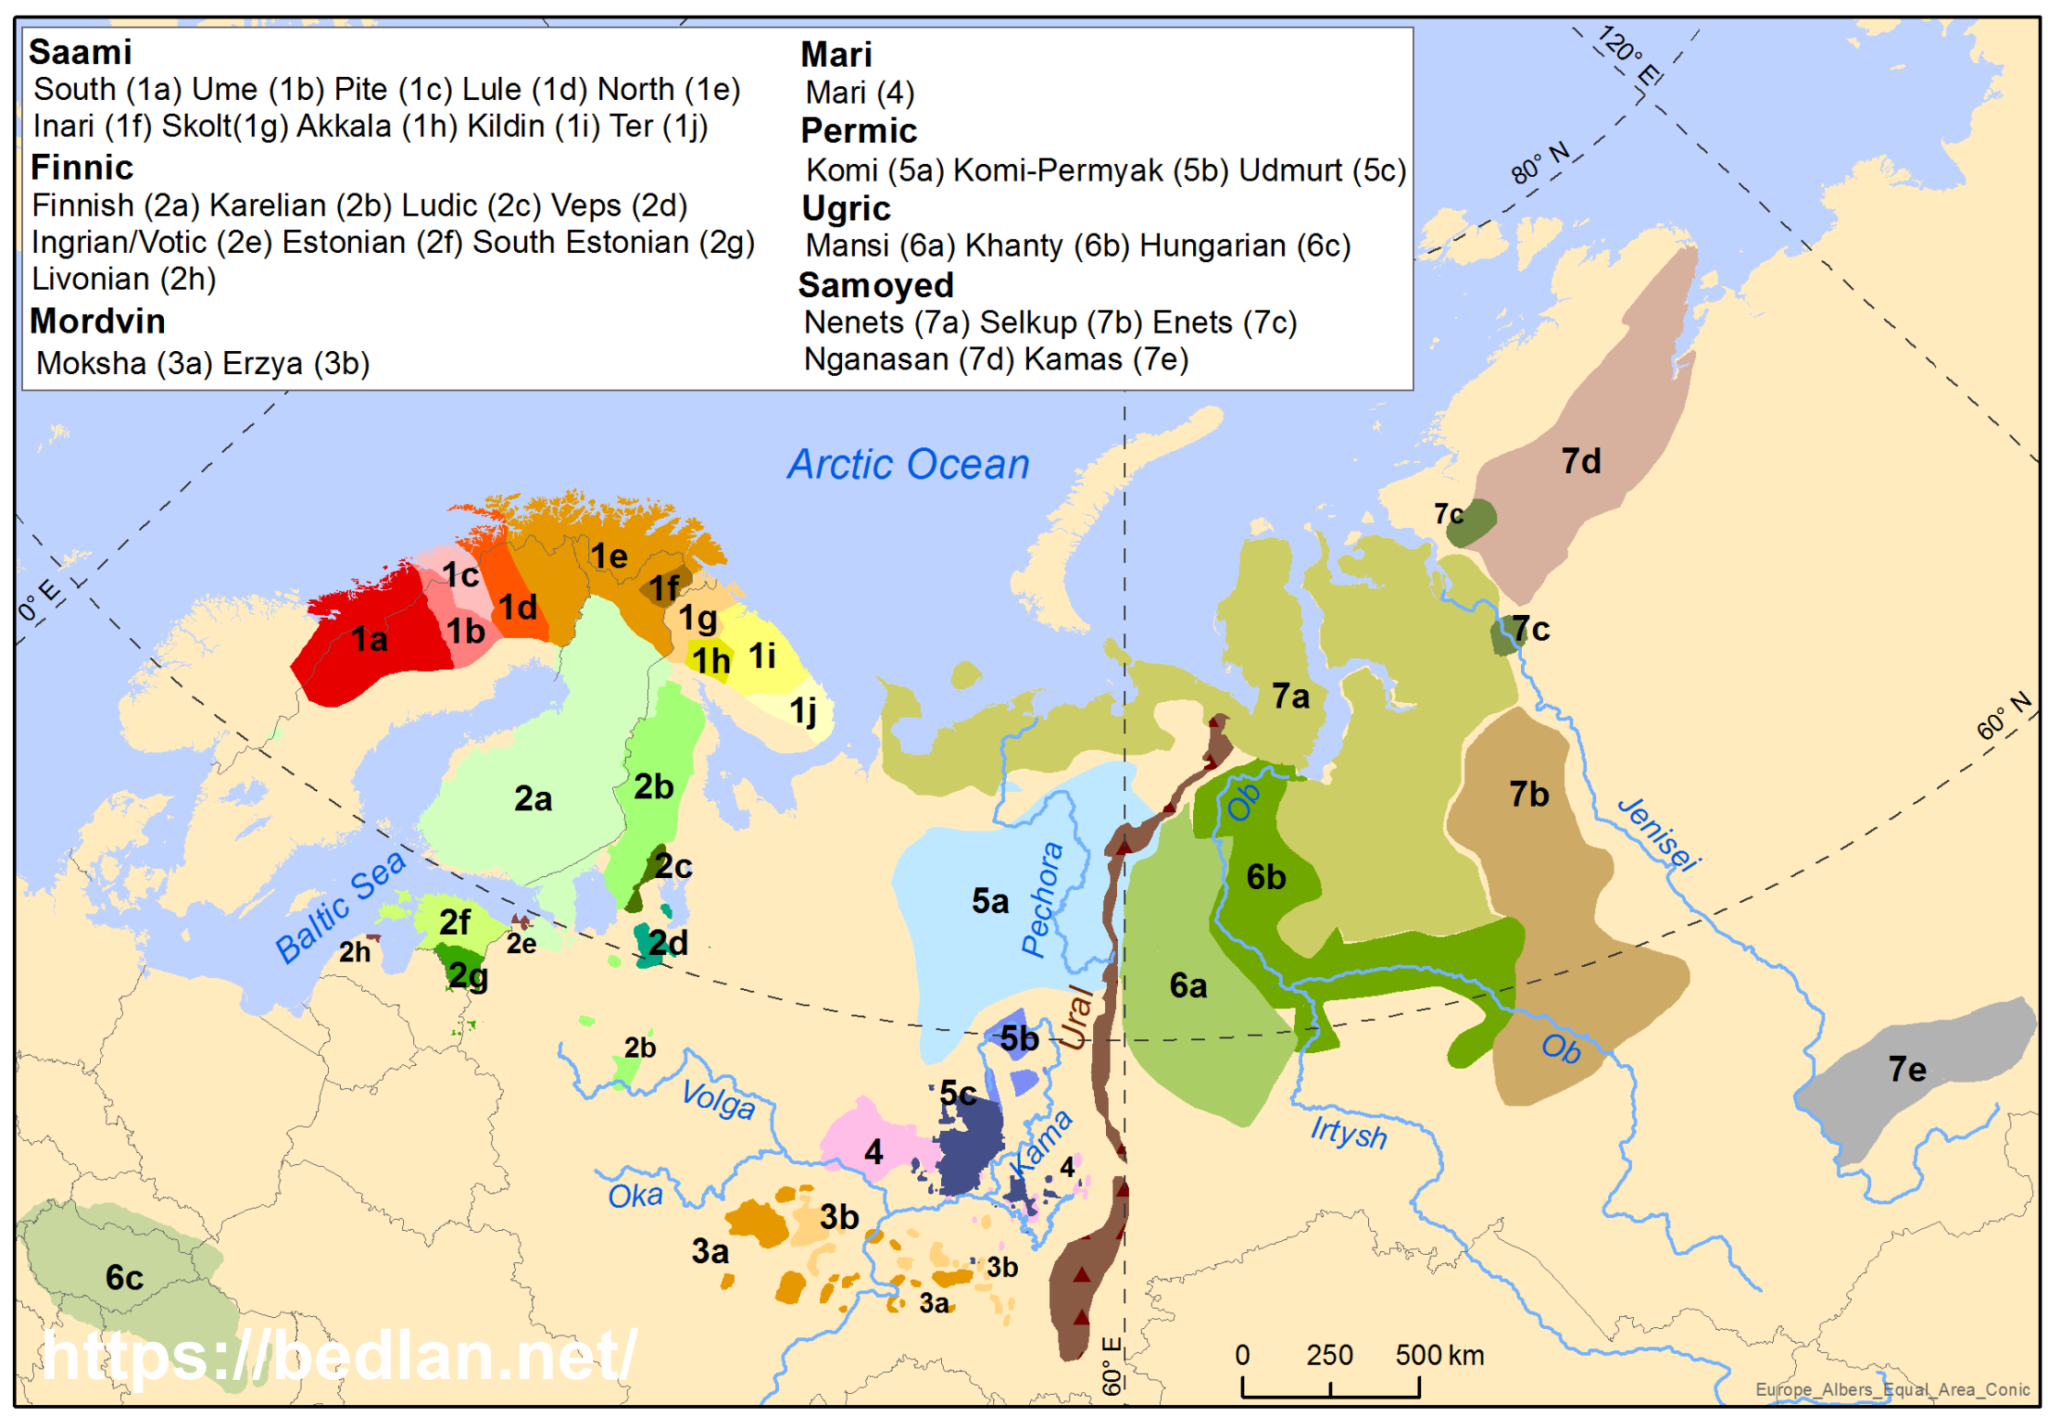
\includegraphics[scale=.15]{uralic-map}
	\end{figure}

\end{frame}

\begin{frame}{Glimpse into sociolinguistics}

	\begin{enumerate}[$\gg$]
		\item Most Uralic languages are endangered
		\item Wikipedia chart based on Russia (2010) and EU (2012 and comparable dates) censuses
	\end{enumerate}
	
	\begin{figure}[H]
		\centering
		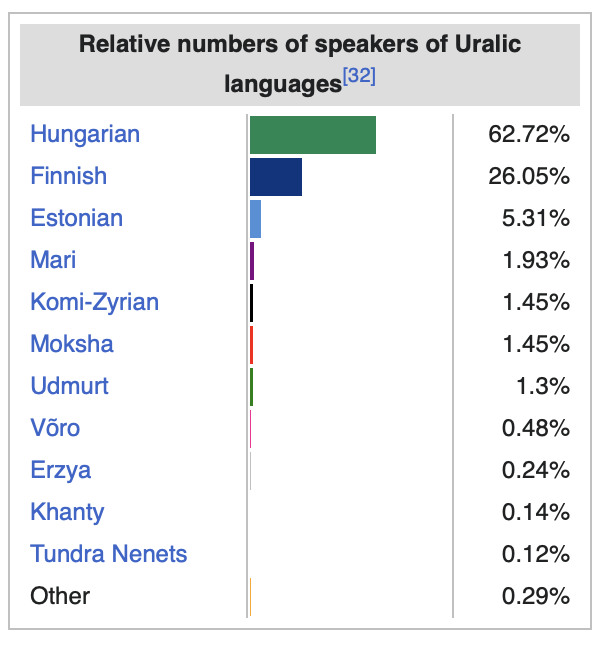
\includegraphics[scale=.5]{wiki-chart}
	\end{figure}

\end{frame}

\begin{frame}{Uralic family}

	\begin{enumerate}[$\gg$]
		\item 42 languages, according to \href{https://www.ethnologue.com/subgroup/1083/}{Ethnologue}
		\item Spoken by approximately 25 million people [\href{https://www.britannica.com/topic/Uralic-languages}{source}]
		\item Largest language is Hungarian ($\sim$17 mil), a lot of minority languages on different levels of endangerement
		\item Branches that can be uncontroversially established \parencite{salminen2002}
			\begin{enumerate}[$\cdot$]
			\normalsize
%			\centering
			\setlength\itemsep{0em}
				\item Finnic
				\item Mari
				\item Mordvin
				\item Permian
				\item Sami
				\item Samoyed
				\item Hungarian, Khanty, Mansi
			\end{enumerate}
	\end{enumerate}

\end{frame}

\begin{frame}{Branches of Uralic}

	\begin{figure}[H]
		\centering
		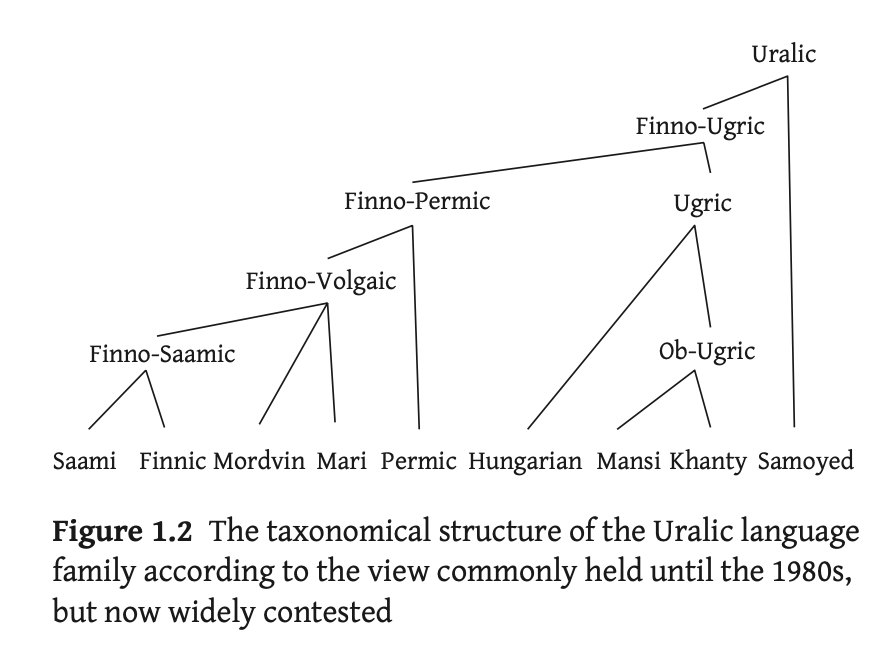
\includegraphics[scale=.65]{uralic-1980s}
		\parencite{aikio2022}
	\end{figure}

\end{frame}

\begin{frame}{Branches of Uralic}

	\begin{enumerate}[$\gg$]
		\item Finnic, Mari, Mordvin, Permic and Saami languages, together with Hungarian, Khanty and Mansi  
		\item ``To sum up the phonological and other evidence for the alleged proto-languages between Proto-Uralic and the level of the basic branches, it can be stated that there is very little of it'' \parencite{salminen2002}
	\end{enumerate}
	
	\begin{figure}[H]
		\centering
		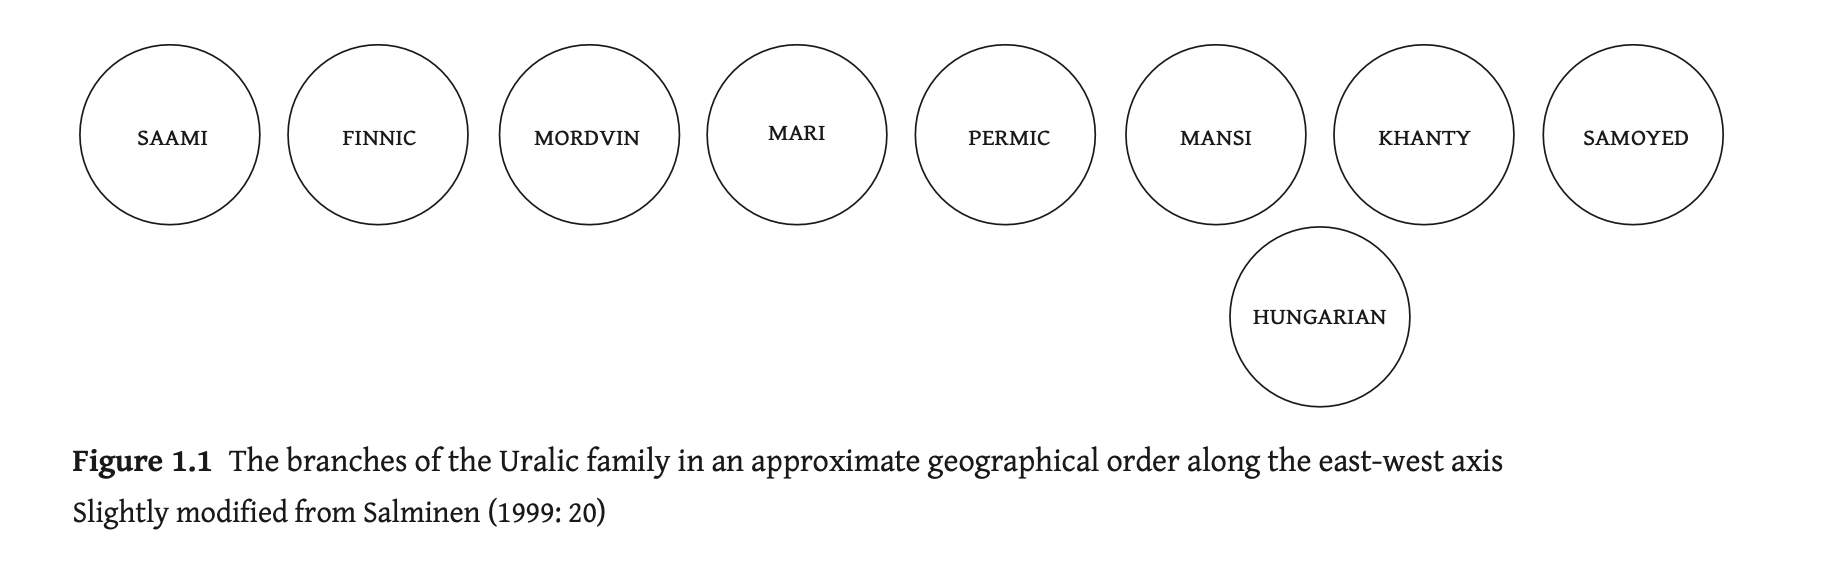
\includegraphics[scale=.37]{uralic-continuum}
		\parencite{aikio2022}
	\end{figure}

\end{frame}

	\section{Branch by branch}

\begin{frame}{Sa(a)mi}

	\begin{enumerate}[$\gg$]
		\item Several Saami languages are now spoken in Norway, Sweden, Finland\\
			North (the biggest of all), South, Inari, Skolt
		\item Only one Saami language left in Russian Federation -- Kildin Saami
	\end{enumerate}
	Most notable common features:

	\begin{enumerate}[$\gg$]
		\item Trochaic stress with unstressable final syllables
		\item Complex vowel quality alternations (historically explicable)
			\pex Kildin Saami vowel alternation \parencite{kert1971}
				\a \emph{jelʹlʹe} \hfill `to live'
				\a \emph{jaλa} \hfill `live.{\Prs}.{\Fsg}'
				\a \emph{jilʹlʹe} \hfill `live.{\Impf}.{\Fsg}'
			\xe
		\item Consonant gradation
	\end{enumerate}

\end{frame}

\begin{frame}{Finnic}

	\begin{enumerate}[$\gg$]
		\item Spoken in Finland, Estonia, North-West Russia and Latvia
		\item A lot of consonant gradation
			\pex Finnish consonant gradation (quantitative; semi-productive)
				\a \emph{pappi} `priest' : \emph{papit} `priests'
				\a \emph{lobbaan} : \emph{lobata} `to lobby'
			\xe
			\pex Karelian consonant gradation (qualitative; \cite{})
				\a \emph{ukko} `old man.{\Nom}' : \emph{ukon} `old man.{\Gen}'
				\a \emph{voassa} `bear.{\Nom}' : \emph{voasan} `bear.{\Gen}'
			\xe
		\item Trochaic stress, primary stress on the first syllable, final syllable unstressed
	\end{enumerate}

\end{frame}

\begin{frame}{Finnic}

	Examples from Karelian \parencite{ryagoev1993}
	\begin{enumerate}[$\gg$]
		\item Vowel harmony
			\pex 
				\a \emph{kala} \hfill `fish'
				\a \emph{nʹ{\"a}g{\"o}} \hfill `face'
			\xe
		\item Vowel length contrast
			\pex
				\a \emph{tuulʹi} \hfill `wind'
				\a \emph{tulʹi} \hfill `fire'
			\xe
	\end{enumerate}

\end{frame}

\begin{frame}{Mordvin}

	\begin{enumerate}[$\gg$]
		\item Spoken in the Mordovia republic and neighbouring regions, European part of Russia
	\end{enumerate}

	\begin{figure}[H]
		\centering
		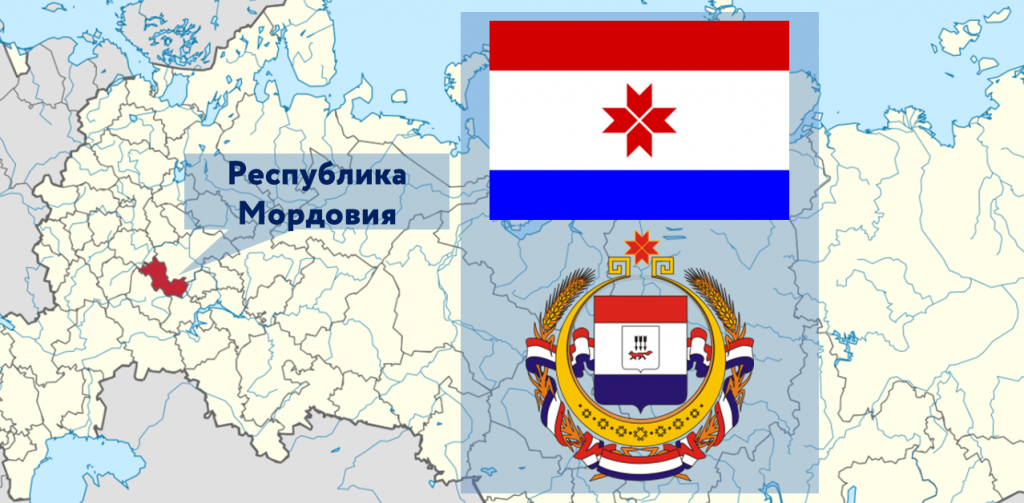
\includegraphics[scale=.4]{mordovia-map}
	\end{figure}

\end{frame}

\begin{frame}{Mordvin}

	\begin{enumerate}[$\gg$]
		\item Moksha and Erzya languages; divided into smaller dialects
		\item Endangered but supported 
	\end{enumerate}
	
	\begin{figure}[H]
		\centering
		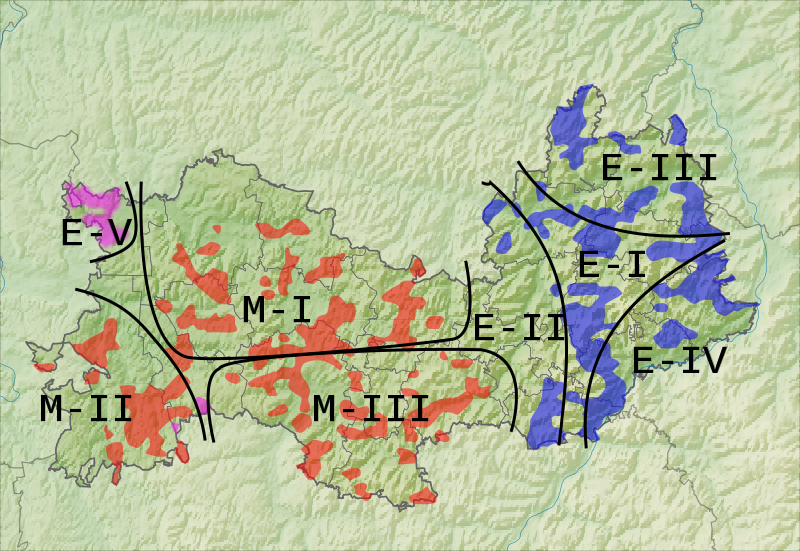
\includegraphics[scale=.3]{moksha-dialects}
	\end{figure}

\end{frame}

\begin{frame}{Mordvin}

	In the Moksha language, as described in \parencite{toldovaetal2018}:

	\begin{enumerate}[$\gg$]
		\item Contrastive palatalisation
			\ex \emph{mar} -- \emph{mar'} \hfill `pile' -- `apple'
			\xe
		\item Contrastive voicing, in sonorants as well (Moksha only)
			\ex \emph{kal} -- \emph{kal̥-n'ə} -- \emph{kal-n'e} \hfill `fish' -- `fish-{\Pl}' -- `fish-{\Fsg}.{\Poss}.{\Pl}'
			\xe
		\item Initial stress, shifted depending on vowel quality:
			\pex
				\a \emph{k{\'a}l̥n'ə} (initial default) \hfill `fish.{\Def}.{\Pl}'
				\a \emph{kuv{\'a}kə} (non-initial shifted) \hfill `long'
			\xe
	\end{enumerate}

\end{frame}

\begin{frame}{Mordvin}

	\begin{enumerate}[$\gg$]
		\item Heaviest possible syllable structure: CCCVCCCC
			\pex Moksha consonant clusters
				\a CCCVCCCC: \emph{kšt'ər'fc't'} \hfill `spin.{\Caus}.{\Pst}.{\Tpl}'
				\a CCCVCCC: \emph{kstikst} \hfill `berry garden.{\Pl}'
				\a CCVCCCC: \emph{bratksc'} \hfill `fraternise.{\Pst}.{\Tsg}'
			\xe
		\item Vowel hiatus is prohibited
			\pex Glide insertion in vowel hiatus
				\a \emph{mu} + \emph{an} $\rightarrow$ \emph{mu-jan} \hfill `find-{\Fsg}'
				\a \emph{jo\v{z}u} + \emph{an} $\rightarrow$ \emph{jo\v{z}u-van} \hfill `smart-{\Fsg}'
			\xe
	\end{enumerate}

\end{frame}

\begin{frame}{Mari}

	\begin{enumerate}[$\gg$]
		\item Mari languages: Meadow Mari and Hill Mari
		\item Spoken in the European part of Russia
	\end{enumerate}
	
	\begin{figure}[H]
		\centering
		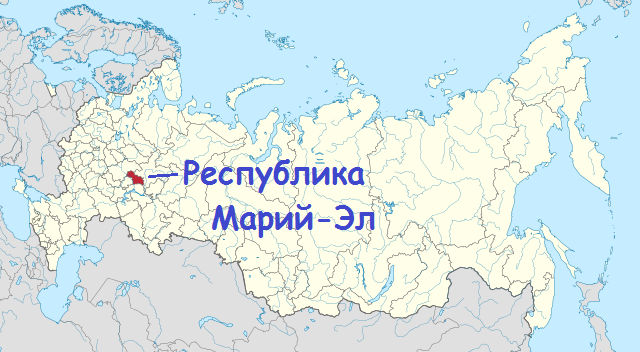
\includegraphics[scale=.6]{mari-el-map}
	\end{figure}
	
\end{frame}

\begin{frame}{Mari}
	
	\begin{enumerate}[$\gg$]
		\item Exception from the regular Uralic trochaic stress pattern
			\pex Penultimate stress is prevalent in Hill Mari \parencite{krasnova2017}
				\a \emph{l\textbf{ə̑}d-aš} \hfill `read-{\Inf}'
				\a \emph{lə̑d-\textbf{ə̑}kt-aš} \hfill `read-{\Caus}.{\Dst}-{\Inf}'
				\a \emph{lə̑d-ə̑kt-\textbf{a}l-aš} \hfill `read-{\Caus}.{\Dst}-{\Att}-{\Inf}'
			\xe
		\item Stress can be contrastive and sometimes has to be lexically encoded
			\pex Contrastive stress in Mari \parencite{kovedyaeva}
				\a \emph{š{\'e}rɣe} \hfill `dear'
				\a \emph{šerɣ{\'e}} \hfill `comb'
			\xe
	\end{enumerate}
	
\end{frame}

\begin{frame}{Mari}
	
	\begin{enumerate}[$\gg$]
		\item Vowel harmony in Hill Mari 
			\pex Front vowels only after front vowels
				\a \emph{arava} \hfill `wagon, wheel'
				\a \emph{ävä} \hfill `mother'
			\xe
			
			\pex~ Non-front vowels only after non-front vowels
				\a \emph{mond-en-äm} \hfill `forget-{\Pret}-{\Fsg}'
				\a \emph{ə̑l-ə̑n-am} \hfill `be-{\Pret}-{\Fsg}'
			\xe
		\item Free distribution only in initial syllables
	\end{enumerate}
	
\end{frame}

%\begin{frame}{Permic}
%
%	\begin{enumerate}[$\gg$]
%		\item Permic languages: Komi and Udmurt
%		\item 
%		\item 
%		\item 
%	\end{enumerate}
%
%\end{frame}
%
%\begin{frame}{Mansi}
%
%	\begin{enumerate}[$\gg$]
%		\item 
%	\end{enumerate}
%
%\end{frame}
%
%\begin{frame}{Hungarian}
%
%	\begin{enumerate}[$\gg$]
%		\item 
%	\end{enumerate}
%
%\end{frame}

\begin{frame}{Khanty}

	\begin{enumerate}[$\gg$]
		\item Spoken in Khanty-Mansi and Yamalo-Nenets okrugs (Western Siberia; Kh-M on the map)
		\item Significant variation between dialects
		\item Traditional occupations: fishing, reindeer herding and hunting
	\end{enumerate}
	
	\begin{figure}[H]
		\centering
		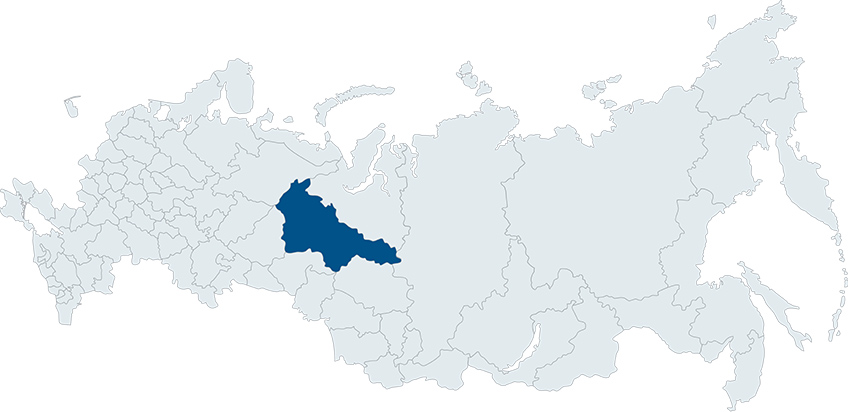
\includegraphics[scale=.3]{khmao-map}
	\end{figure}
	
\end{frame}

\begin{frame}{Khanty dialects}
	
	\begin{figure}[H]
		\centering
		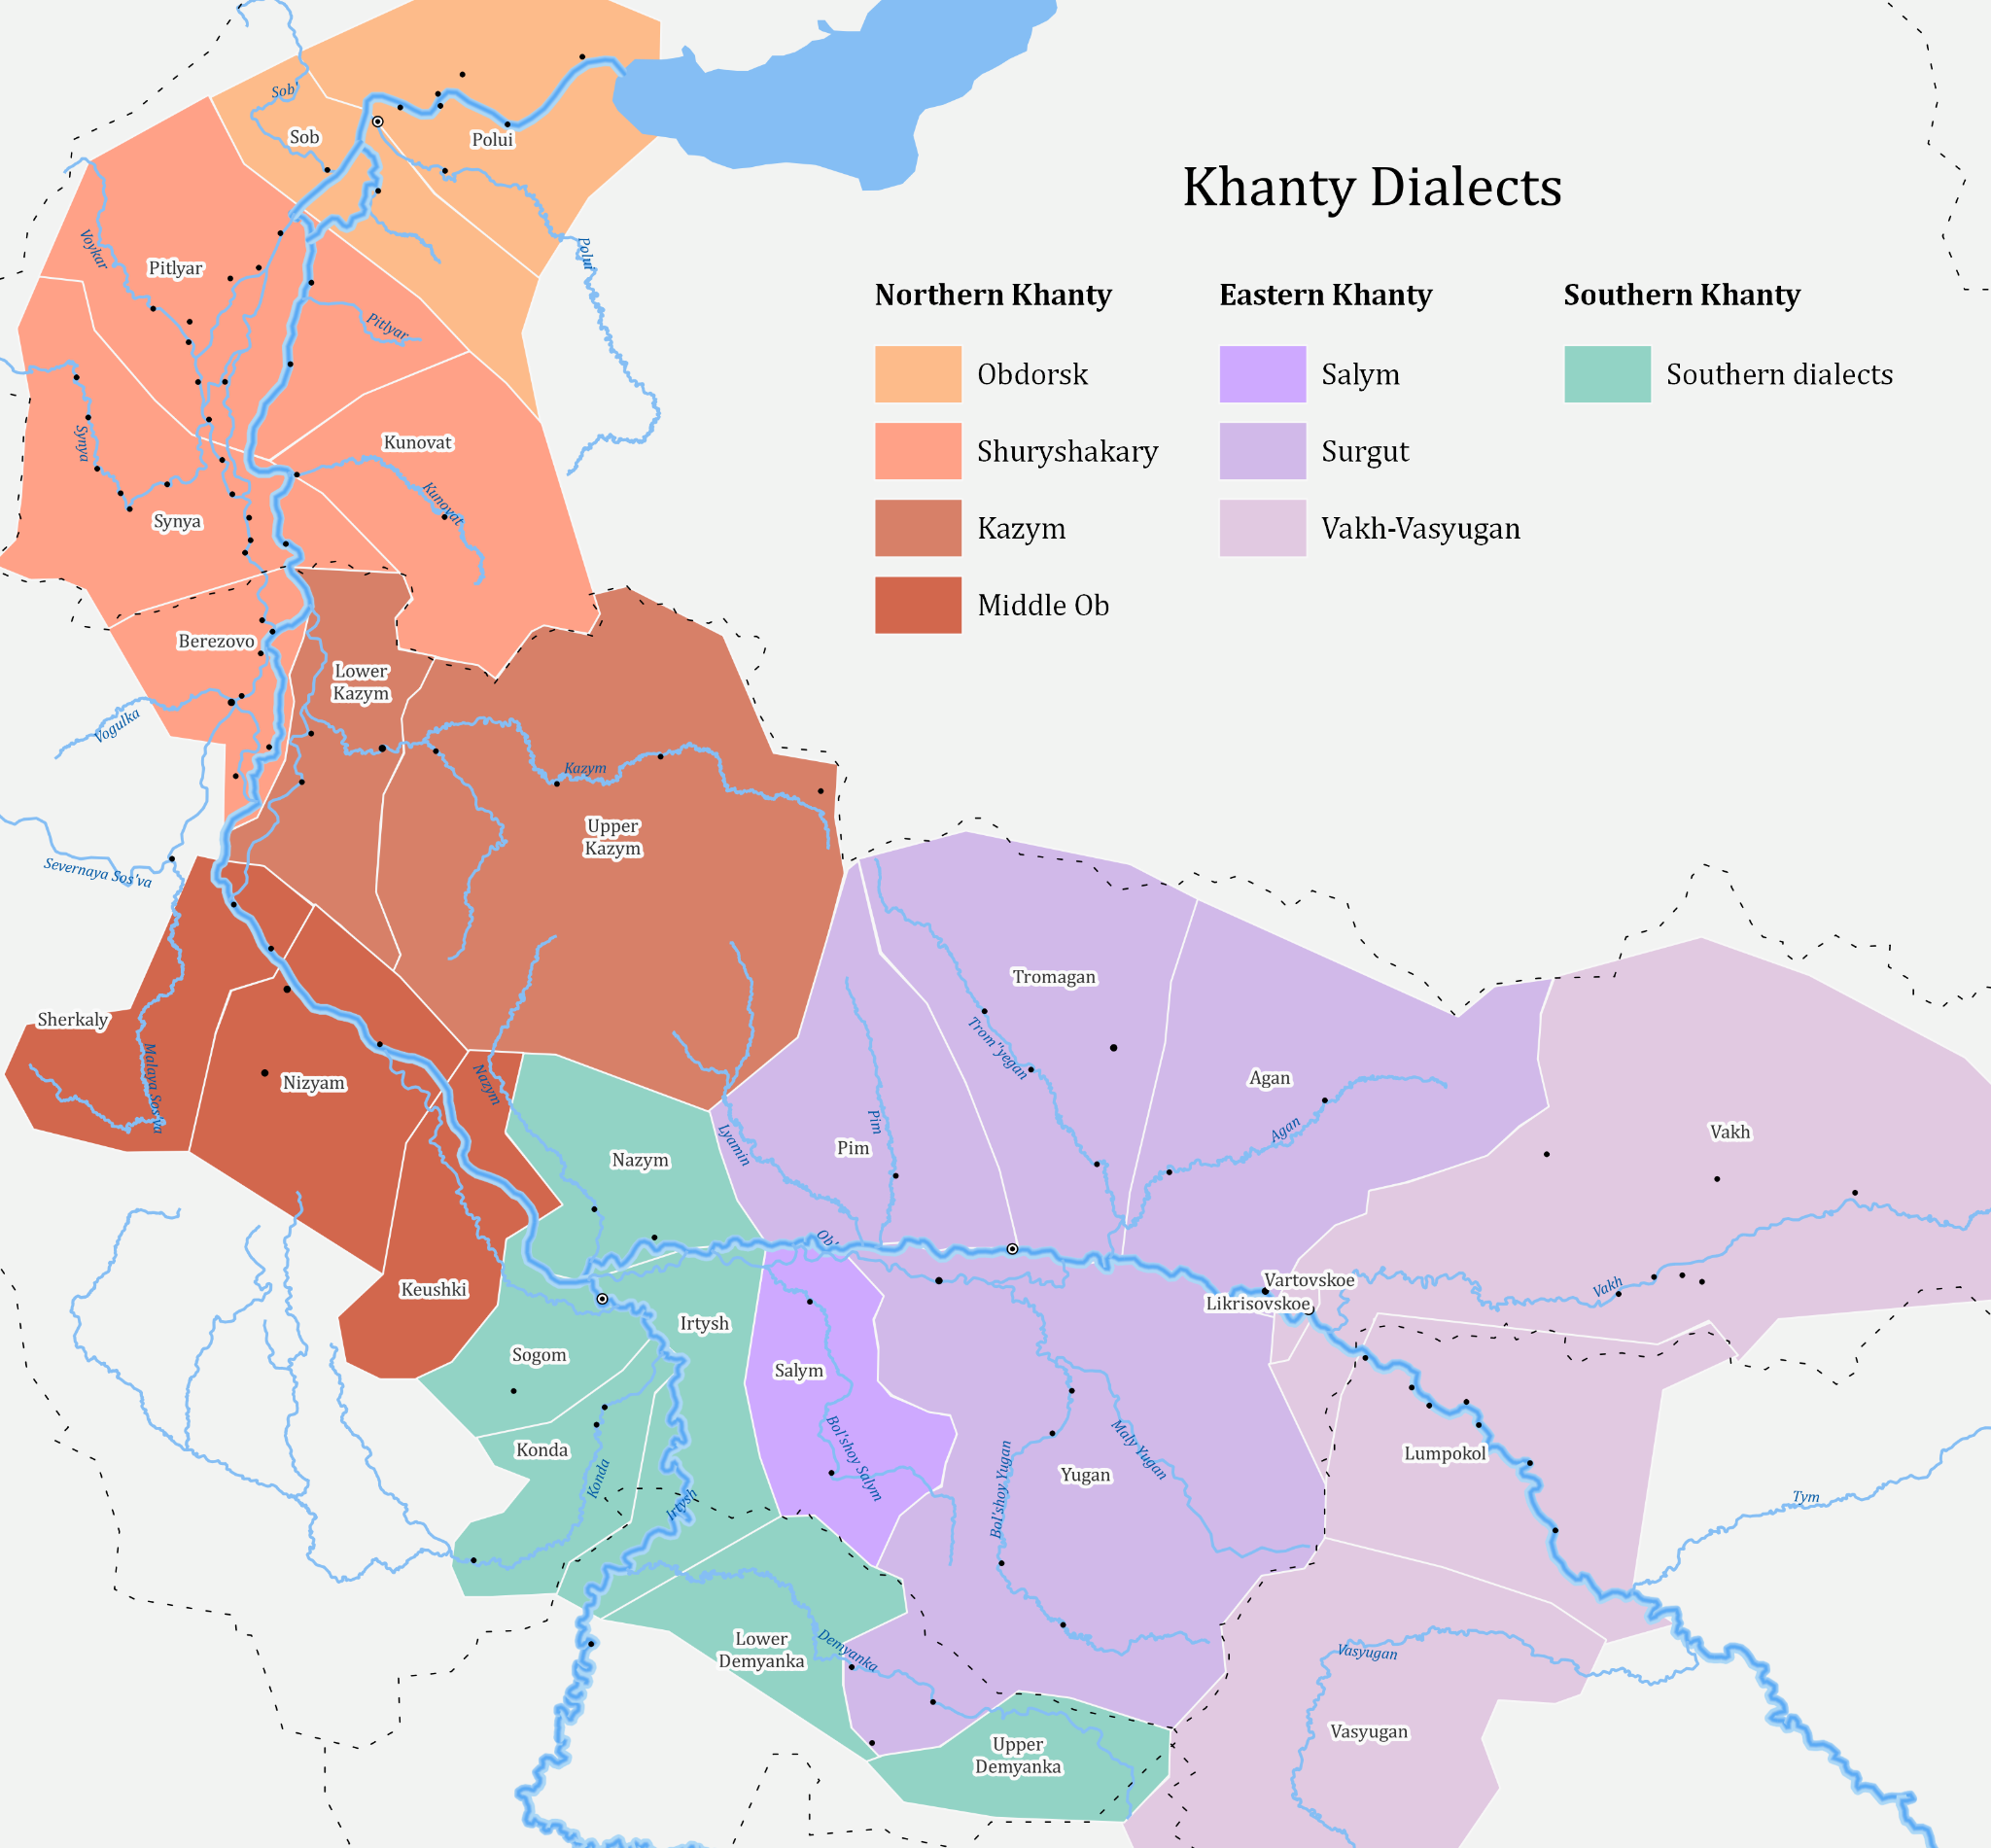
\includegraphics[scale=.12]{khanty-dialects}
	\end{figure}

\end{frame}

\begin{frame}{Khanty}

	\begin{enumerate}[$\gg$]
		\item Voiceless fricative [ɬ] typed as /λ/
		\item No voicing contrast in stops
			\pex Russian loanwords in Kazym Khanty
				\a \emph{danila} (Rus) $\rightarrow$ \emph{tańλa} (Kh) \hfill (Daniel)
				\a \emph{grigorij} (Rus) $\rightarrow$ \emph{kirkɵr} (Kh) \hfill (Gregory)
			\xe
		\item (C)V(C)(C) syllable structure
			\pex Epenthesis to rescue initial clusters in Kazym Khanty
				\a \emph{kni\v{z}ka} (Rus) $\rightarrow$ \emph{kinška} (Kh) \hfill `book'
				\a \emph{škola} (Rus) $\rightarrow$ \emph{aškola} (Kh) \hfill `school'
			\xe
	\end{enumerate}

\end{frame}

\begin{frame}{Khanty}

	\begin{enumerate}[$\gg$]
		\item Schwa is subject to vowel-zero alternations in some morphemes
			\pex Surface realisations of the suffix \emph{-əmən} `{\Fdu}'
				\a \emph{orət-λ-əmn} \hfill `drag-{\Npst}-{\Fdu}'
				\a \emph{pɵrλə-s-mən} \hfill `soar-{\Pst}-{\Fdu}'
			\xe 
		\item Trochaic stress
			\pex Khanty stress pattern
				\a \emph{ˈλaraś} \hfill \emph{λaraś} `box'
				\a \emph{ˈλaraˈśɛma} \hfill \emph{λaraś-ɛm-a} `box-{\Poss}.{\Fsg}-{\Dat}'
				\a \emph{ˈλaraśa} \hfill \emph{λaraś-a} `box-{\Dat}'
			\xe 
	\end{enumerate}

\end{frame}

\begin{frame}{Samoyed}

	\begin{enumerate}[$\gg$]
		\item Samoyed languages: Nganasan, Enets, Nenets, Selkup
		\item Nenets languages: Tundra Nenets (TN) and Forest Nenets (FN)
		\item Yamal-Nenets okrug on the map
	\end{enumerate}
	
	\begin{figure}[H]
		\centering
		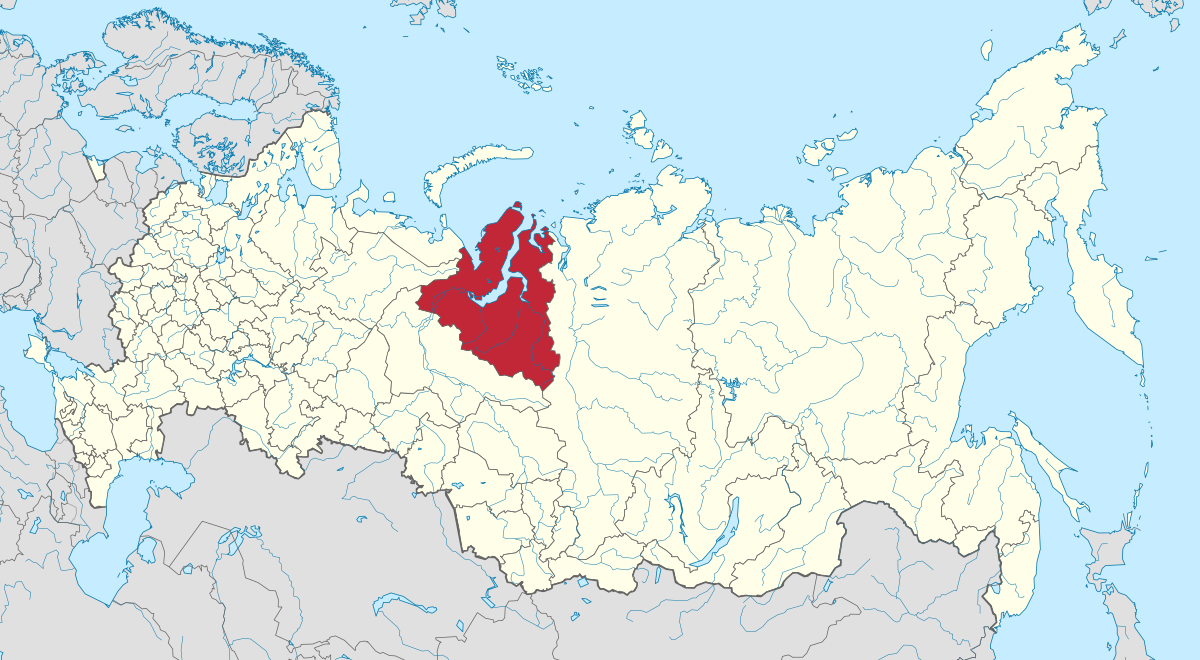
\includegraphics[scale=.23]{yanao-map}
	\end{figure}

\end{frame}

%\begin{frame}{Nenets}
%	
%	\begin{figure}[H]
%		\centering
%		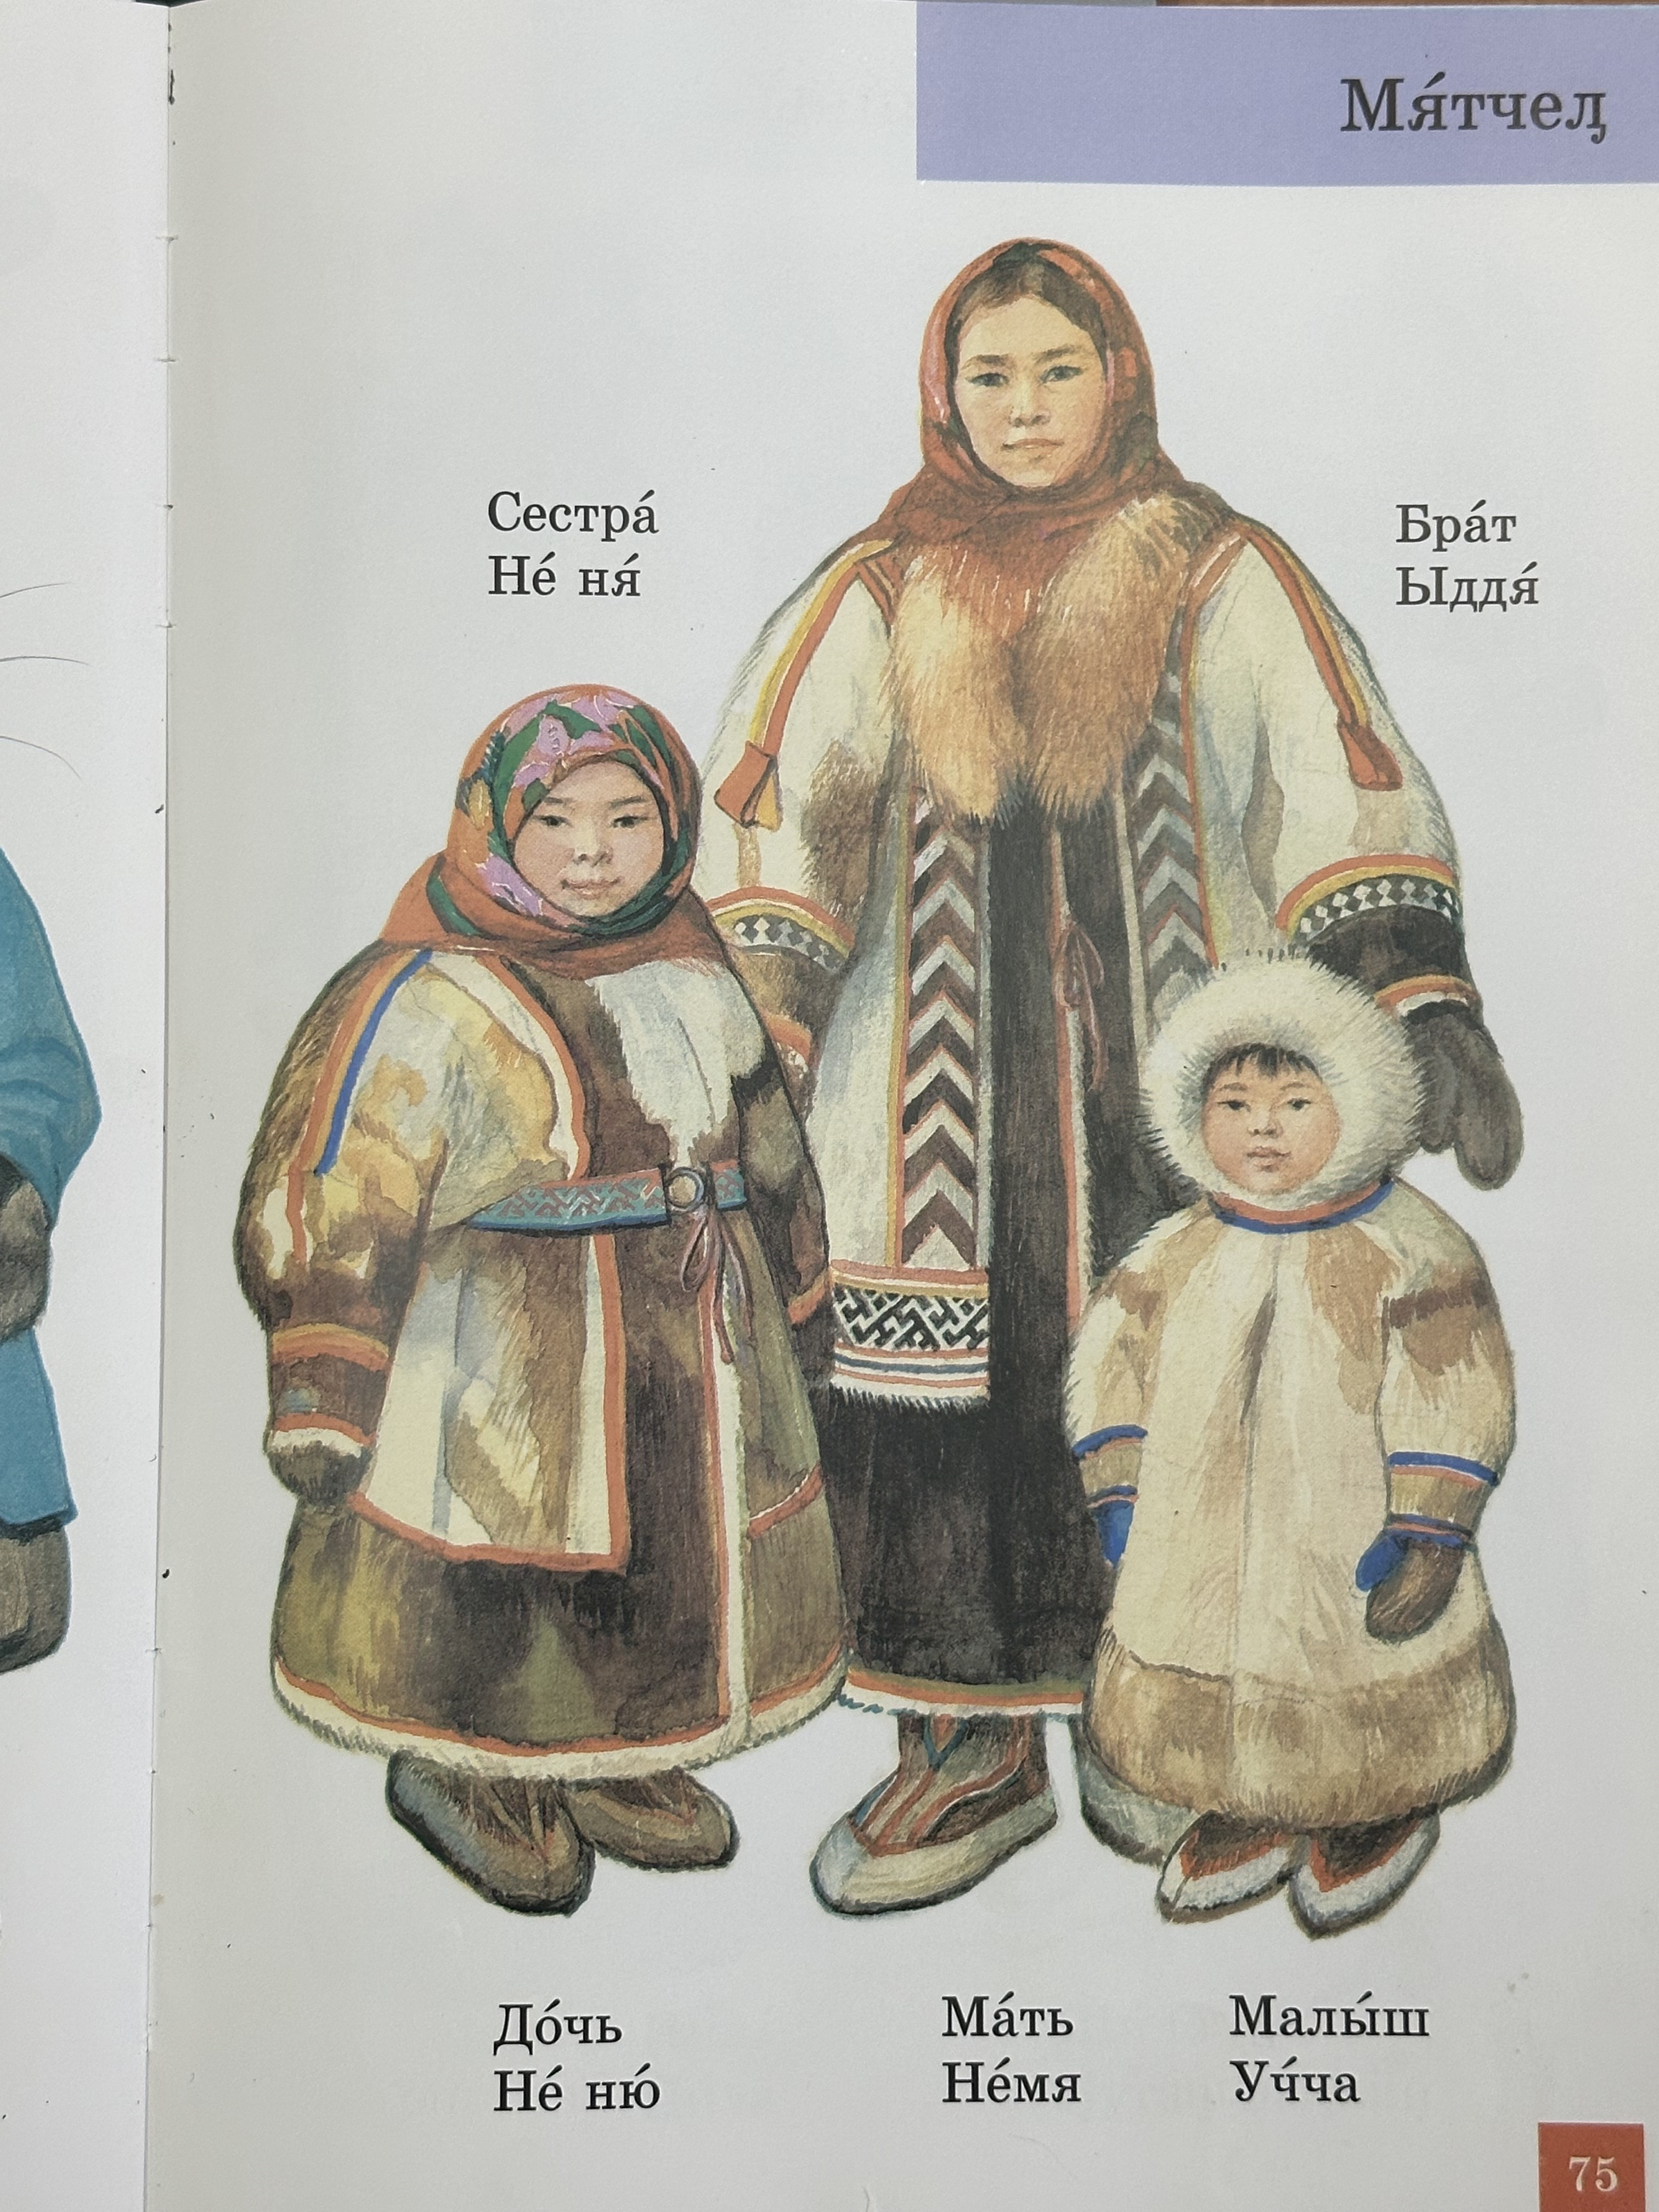
\includegraphics[scale=.055]{nenets-women}
%	\end{figure}
%
%\end{frame}

\begin{frame}{Nenets}
	
	In Nenets, as described by \citeay{sammallahti1974}, \citeay{salminen2007}, \citeay{burkova2022}:
	\begin{enumerate}[$\gg$]
		\item Contrastive vowel length in FN
			\ex \emph{kăta} -- \emph{kata} \hfill `fingernail' -- `grandmother'
			\xe
		\item Only preserved in stressed syllables
		\item Over-short vowel schwa, occasionally exponed suprasegmentally
			\pex Schwa in FN -- /°/
				\a \emph{ka-λ°} [kaλĭ] \hfill `ear-{\Poss}.{\Ssg}'
				\a \emph{kăλ°} [kăλλ] \hfill `knife'
				\a \emph{kinʹiw°} [kinʹ{\'i}w] \hfill `cat'
			\xe
	\end{enumerate}

\end{frame}

\begin{frame}{Nenets}
	
	\begin{enumerate}[$\gg$]
		\item No voicing contrast in consonants
		\item Contrastive palatalisation (examples from FN)
			\pex 
				\a \emph{păj°} -- \emph{pʹaj} \hfill `crooked' -- `wooden'
				\a \emph{tĭ} -- \emph{čiλ°} \hfill `reindeer' -- `cloud'
			\xe
		\item Occasional consonant gradation effects in FN
			\pex Forest Nenets durative \parencite[p. 359]{salminen2007}
				\a \emph{kata-pʹo-} \hfill `kill-{\Dur}'
				\a \emph{ta-mʹpʹo-} \hfill `bring-{\Dur}'
			\xe
	\end{enumerate}

\end{frame}

\begin{frame}{Nenets}

	\begin{enumerate}[$\gg$]
		\item Vowel harmony in VxV contexts
			\pex FN /a ă °/ subject to vowel harmony
				\a \emph{tŏ} + \emph{xăna} $\rightarrow$ \emph{toxona} \hfill `lake-{\Loc}'
				\a \emph{dʹiλʹi} + \emph{xăna} $\rightarrow$ \emph{dʹiλʹixina} \hfill `month-{\Loc}'
			\xe
		\item Basic syllable structure is CV(C)
		\item Trochaic non-final stress
			\pex TN stress pattern
				\a \emph{tataŋata} [ˈta.ta.ˈŋa.ta] \hfill `he’s exchanging'
				\a \emph{wedʹaʔku} [ˈwe.dʹaʰ.ku] \hfill `dog'
			\xe 
	\end{enumerate}

\end{frame}

\begin{frame}{Characteristic features of Uralic}

	Vowel systems:
	\begin{enumerate}[$\gg$]
		\item Contrastive vowel length
		\item Vowel harmony (Hungarian, Mari, Samoyed)
		\item Phonologically contrastive tone is not observed
	\end{enumerate}
	
\vfill
	
	Consonants:
	\begin{enumerate}[$\gg$]
		\item Contrastive palatalisation (Saami, Khanty, Moksha, Nenets; lost in Finnic)
		\item Occasionally lacking contrastive voicing; curious interaction with Russian
		\item A range of possible consonant clusters: from almost none (Khanty, Nenets) to really big (Moksha)
	\end{enumerate}

\end{frame}

\begin{frame}{Characteristic features of Uralic}

	Stress patterns:
	
	\begin{enumerate}[$\gg$]
		\item Initial primary stress, secondary stress on odd non-final syllables
		\item Affected by vowel quality in Moksha
		\item Interacts with vowel-zero alternations in Khanty and Forest Nenets
		\item Lexical accent in Mari
		\item Phonologically contrastive tone is not observed
	\end{enumerate}

\end{frame}

\begin{frame}{Roadmap}

\begin{table}[]
\begin{tabular}{llp{.37\textwidth}}
\toprule
          & \textbf{Languages}                   & \textbf{Topics}                                           \\
          \midrule
\textbf{Tuesday}   & Finnish, Estonian, Saami    & Consonant gradation                              \\
\addlinespace[0.2cm]
\textbf{Wednesday} & Moksha                      & Hiatus resolution, stress                        \\
\addlinespace[0.2cm]
\textbf{Thursday}  & Khanty (Kazym d.)      & Vowel-zero alternations, stress                  \\
\addlinespace[0.2cm]
\textbf{Friday}    & Forest Nenets (Pur d.) & Vowel length, stress, schwa, consonant gradation, vowel harmony \\
\bottomrule
\end{tabular}
\end{table}
\end{frame}

\begin{frame}{Phonological framework}

	\begin{enumerate}[$\gg$]
		\item Analyses will be couched in Strict CV
		\item Before a theoretical analysis, framework-free generalisations will be established
		\item Materials available:
			\begin{enumerate}[$\cdot$]
			\normalsize
%			\centering
			\setlength\itemsep{0em}
				\item {[\href{link}{datasets}]}
				\item {[\href{link}{last week's class handouts}]}
			\end{enumerate}
	\end{enumerate}

\end{frame}

%\begin{frame}{}
%\end{frame}
%
%\begin{frame}{}
%\end{frame}
%
%\begin{frame}{}
%\end{frame}
%
%\begin{frame}{}
%
%	\begin{enumerate}[$\gg$]
%		\item 
%	\end{enumerate}
%
%\end{frame}

\begin{frame}[allowframebreaks]
\frametitle{References}
%\bibliography{ref}
\printbibliography
\end{frame}

\end{document}